
\setcounter{chapter}{2}
\chapter{Implementation of a Flexible Data Analysis Library for Hybrid X-ray Particle Detectors }
\minitoc %insert la minitoc
\graphicspath{{Chapitre3/figures/}}

%\DoPToC
%==============================================================================
\pagestyle{fancy}
\fancyhf{}
\fancyhead[R]{\bfseries\rightmark}
\fancyfoot[R]{\thepage}
\renewcommand{\headrulewidth}{0.5pt}
\renewcommand{\footrulewidth}{0pt}
\renewcommand{\chaptermark}[1]{\markboth{{\chaptername~\thechapter. #1 }}{}}
\renewcommand{\sectionmark}[1]{\markright{\thechapter.\thesection~ #1}}

\begin{spacing}{1.2}

    %==============================================================================
    \section*{Introduction}
    In this chapter we will go through the implementation and design choices for each module.

    \section{Project Setup}
    \subsection{Project Structure}
    \begin{figure}[hb]
        \centering
        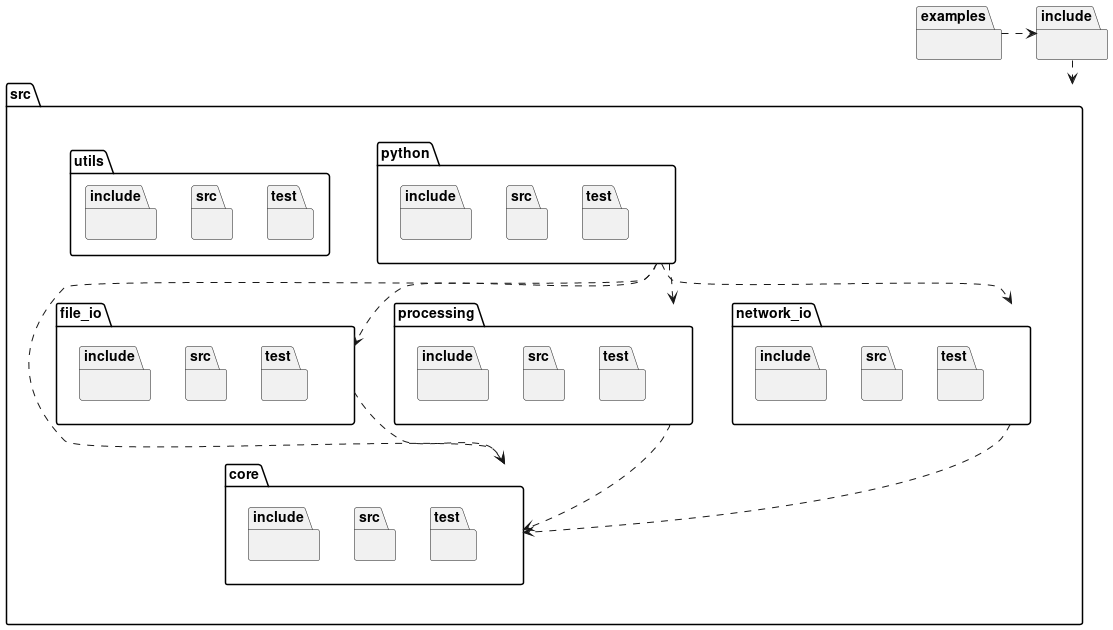
\includegraphics[width=0.8\textwidth]{Chapitre3/figures/folders.png}
        \caption{Project folder structure}
        \label{fig:folders}
    \end{figure}
    The folder structure of the project is shown in Figure \ref{fig:folders}. The file hierarchy
    is based on the Pitchfork project structure recommendations \cite{pitchfork}.
    The project is composed of a include folder containing the header files,
    a src folder containing the source files,
    an examples folder containing the examples.
    The root directory of the project contains a CMakeLists.txt file which is used to build the project.
    Each module has its own folder in the src directory.
    For example the core module has include, src and test folders inside it.




    \subsection{Build System}
    The project uses CMake as the build system. CMake is a cross-platform build system that
    generates native build files for the platform of your choice. It is a powerful tool that
    can be used to build, test and package software. The CMakeLists.txt file in the root directory
    of the project is used to configure the project. Each module also has its own CMakeLists.txt
    file which is used to configure the module and build the sources files and tests. CMake will compile
    each module independently as static libraries and link them together to create the final
    executables or share objects.\\

    In this project CMake is also used to manage the dependencies. The project uses external
    libraries such as ZeroMQ, FMT, Catch2... CMake downloads and builds these libraries
    automatically. This is done using the FetchContent module in CMake. The FetchContent module
    allows to download and build external projects at configure time.

    \subsection{Version Control}
    The project uses Git as the version control system. Git is a distributed version control system
    that allows tracking changes in the source code. It is a powerful tool that allows multiple people
    to work on the same project at the same time.\\

    The remote repository is hosted on GitHub. GitHub is a web-based platform that provides
    hosting for software development version control using Git. It also provides collaboration
    features such as bug tracking, feature requests, task management and wikis for every project.
    Pull requests are used to merge changes from one branch to another. This allows reviewers
    to check the code before it is merged into the main branch.\\



    \subsection{Testing and Continuous Integration}
    The project uses Catch2 as the testing framework. Catch2 is a modern, C++-native, header-only,
    test framework for unit-tests. It is easy to use and provides a lot of features such as
    BDD-style testing, test cases, sections, assertions, tags, test fixtures, test cases
    and test suites.\\

    Each module has its own test folder containing the test files. The test files are compiled
    into a test executable which is run to test the module. The test executable is built using
    the CMakeLists.txt file in the test folder of the module. A single test executable is built
    for the whole library which runs all the tests of the submodules. Tags can be used to run or exclude
    specific groups of tests.\\

    Continuous integration is used to automatically build and test the project. GitHub Actions
    is used to run the tests on each push to the repository. The tests are run on multiple
    platforms including Windows, Linux and MacOS. And different configurations are used such
    as Debug and Release, with and without Python bindings, download dependencies with CMake or use system libraries...
    Furthermore, the code is checked for formatting using clang-format and for linting checks using clang-tidy.
    Linting checks are used to find potential bugs and code smells in the code.\\



    \subfile{Chapitre3/part1.tex}

    \section{Processing Module Implementation}
    \begin{figure}
        \centering
        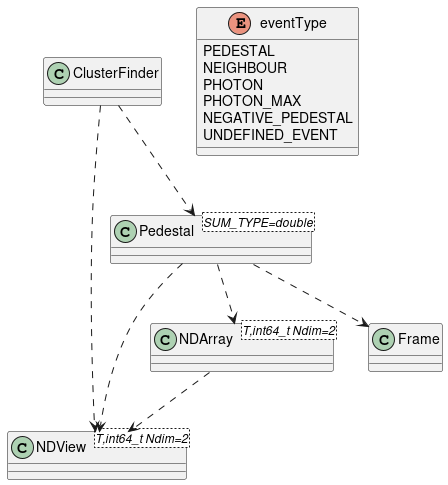
\includegraphics[width=0.8\textwidth]{Chapitre3/figures/processing_class.png}
        \caption{Processing module}
        \label{fig:processing}
    \end{figure}

    The processing module contains the classes and algorithms used to process the data.
    The class diagram of the processing module is shown in Figure \ref{fig:processing}.
    Currently two data processing algorithms are implemented.

    \subsection{Pedestal class}

    The pedestal algorithm is used for preprocessing the incoming frame data. Detectors have a
    background signal that is present even when no particles are detected. This background signal
    can be the still image of the sample. The Pedestal substraction algorithm is used to remove
    this background signal and help in the detection of key meaningful signals. The Pedestal class
    is used to calculate the pedestal values for each pixel. Usually the pedestal values are
    calculated by taking the average of the last N frames. However, in our case we a frame of data
    can have 1024x1024 pixels keeping track of the last N frames would be memory intensive i.e
    $O(N)$ in memory.
    In order to store the last 1000 frames for the average $1024*1024*1000*4 = 4GB$  of memory would be needed.
    Instead we keep track of the sum of the last N frames and with each new frame we subtract the
    average of the last N frames and add the new frame.
    \begin{equation}
        \text{Sum}_i = \text{Sum}_{i-1} - \frac{\text{Sum}_{i-1}}{N} + \text{Frame}_i
    \end{equation}
    \begin{equation}
        \text{Pedestal}_i = \frac{\text{Sum}_i}{N}
    \end{equation}

    This way we only need to store the sum of the last N frames
    which is $1024*1024*4 = 4MB$ of memory.  In addition this method is faster, more stable
    and $O(1)$ in terms of memory and time complexity.


    \subsection{ClusterFinder class}
    After substracting the pedestal values from the incoming frame data, the next step is to
    find the clusters of pixels that are hit by the incoming particles. For photon particles
    a fixed size cluster of 2x2 or 3x3 is used as a sliding window to find the appropriate   particle hits.
    For electrons, as they usually leave a trail behind, a flood fill algorithm is used to find the
    clusters of adjacent pixels that are hit by the incoming particles.\\


    \section{Python Bindings Implementation}
    Writing python code is a lot of fun and very productive. It is a high-level language that is
    easy to learn and use. It is also very popular in the scientific community. It is used for
    data analysis, machine learning, artificial intelligence, web development, automation and many more.

    However, Python is an interpreted language and it is very dynamic. this makes it slower than
    compiled languages like C++. \\

    On the other hand, C++ is a compiled language that is very fast and efficient. It is used to
    write high-performance code that is used in games, operating systems, databases, web servers
    , financial systems and many more.

    It is also very complicated and hard to learn and use. It is strongly typed and has a lot of
    boilerplate code.\\

    Ideally, we would like to write the core of our library in C++ and then use it in Python.
    This is where Python bindings come in. Python bindings are used to expose C++ code to Python.
    There are many ways to create Python bindings such as SWIG, Boost.Python, pybind11, ctypes, CFFI...

    In this project, we use pybind11 to create the Python bindings. pybind11 is a lightweight header-only
    library that exposes C++ code to Python.
    It is influenced by the Boost.Python library, But it presents itself as bloat free alternative.
    It is easy to use and provides a lot of features such as
    automatic type conversion, exception handling, class inheritance, function overloading, lambda functions and
    integrates NumPy support.

    pybind11 is heavily used in numerical/ML libraries such as scipy, Tensorflow, JAX, Pytorch\dots\\

    The pybind11 creates an extension module that can be imported in Python. The extension module
    contains the C++ code that is exposed to Python. After compiling and linking pybind11 produces
    a dynamic library (dynamic load) that can be used by Python. The dynamic library is loaded
    at runtime and the C++ code is executed in the Python interpreter.\\

    \begin{lstlisting}[language=C++, caption=Example of a C++ binding for the Frame class,label=lst:frame_binding]
py::class_<Frame>(m, "Frame", py::buffer_protocol())
    .def(py::init<std::byte *, int64_t, int64_t, Dtype>())
    .def(py::init<int64_t, int64_t, Dtype>())
    .def_property_readonly("rows", &Frame::rows)
    .def_property_readonly("cols", &Frame::cols)
    .def_property_readonly("bitdepth", &Frame::bitdepth)
    .def_property_readonly("size", &Frame::bytes)
    .def_property_readonly("data", &Frame::data, py::return_value_policy::reference)
    .def_buffer([](Frame &f) -> py::buffer_info {
        Dtype dt = f.dtype();
        return {
            f.data(),                           /* Pointer to buffer */
            static_cast<int64_t>(dt.bytes()),   /* Size of one scalar */
            dt.format_descr(),                  /* Python struct-style format descriptor */
            2,                                  /* Number of dimensions */
            {f.rows(), f.cols()},               /* Buffer dimensions */
            {f.cols() * dt.bytes(), dt.bytes()} /* Strides (in bytes) for each index */
        };
});

        
    \end{lstlisting}

    Listing \ref{lst:frame_binding} shows an example of a C++ binding for the Frame class.
    \lstinline|.def()| method is used to define a class method. In the example, we defined 
    the constructor with it. \lstinline|.def_property_readonly()| is used to define a read-only property.
    \lstinline|.def_buffer()| is used to define a buffer protocol. The buffer protocol is used to expose
    the data of the Frame class to Python. This protocol is very useful when working with NumPy arrays 
    as it allows us to convert a Frame object to a NumPy array with or without copying the data.\\

    \begin{lstlisting}[language=Python, caption=Example of using the Frame class in Python,label=lst:frame_python]
import numpy as np # import numpy
import aare        # import the aare library

frame = aare.Frame(1024, 1024, aare.Dtype.UINT16) # create a frame object
rows = frame.rows # get the number of rows
array = np.array(frame.data, copy=False) # convert the frame object to a numpy array
    \end{lstlisting}

    Listing \ref{lst:frame_python} shows an example of using the Frame class in Python.
    As we can see the Frame class is used as a normal Python class. Furthermore, we can 
    manipulate the data of the Frame object as a NumPy array. This is very useful as it allows
    us to use the Frame object with other libraries that use NumPy arrays.\\


    \section*{Conclusion}
    In this chapter, we went through the implementation of the project. We discussed the 
    project setup and we dived deep into the details of the implementation. We dived into
    the design choices that were made in order to juggle between performance, flexibility, 
    and usability. 

    %==============================================================================
\end{spacing}
